% Requires graphicx. Paths assume compilation from repository root.
\begin{figure*}[t]
\centering
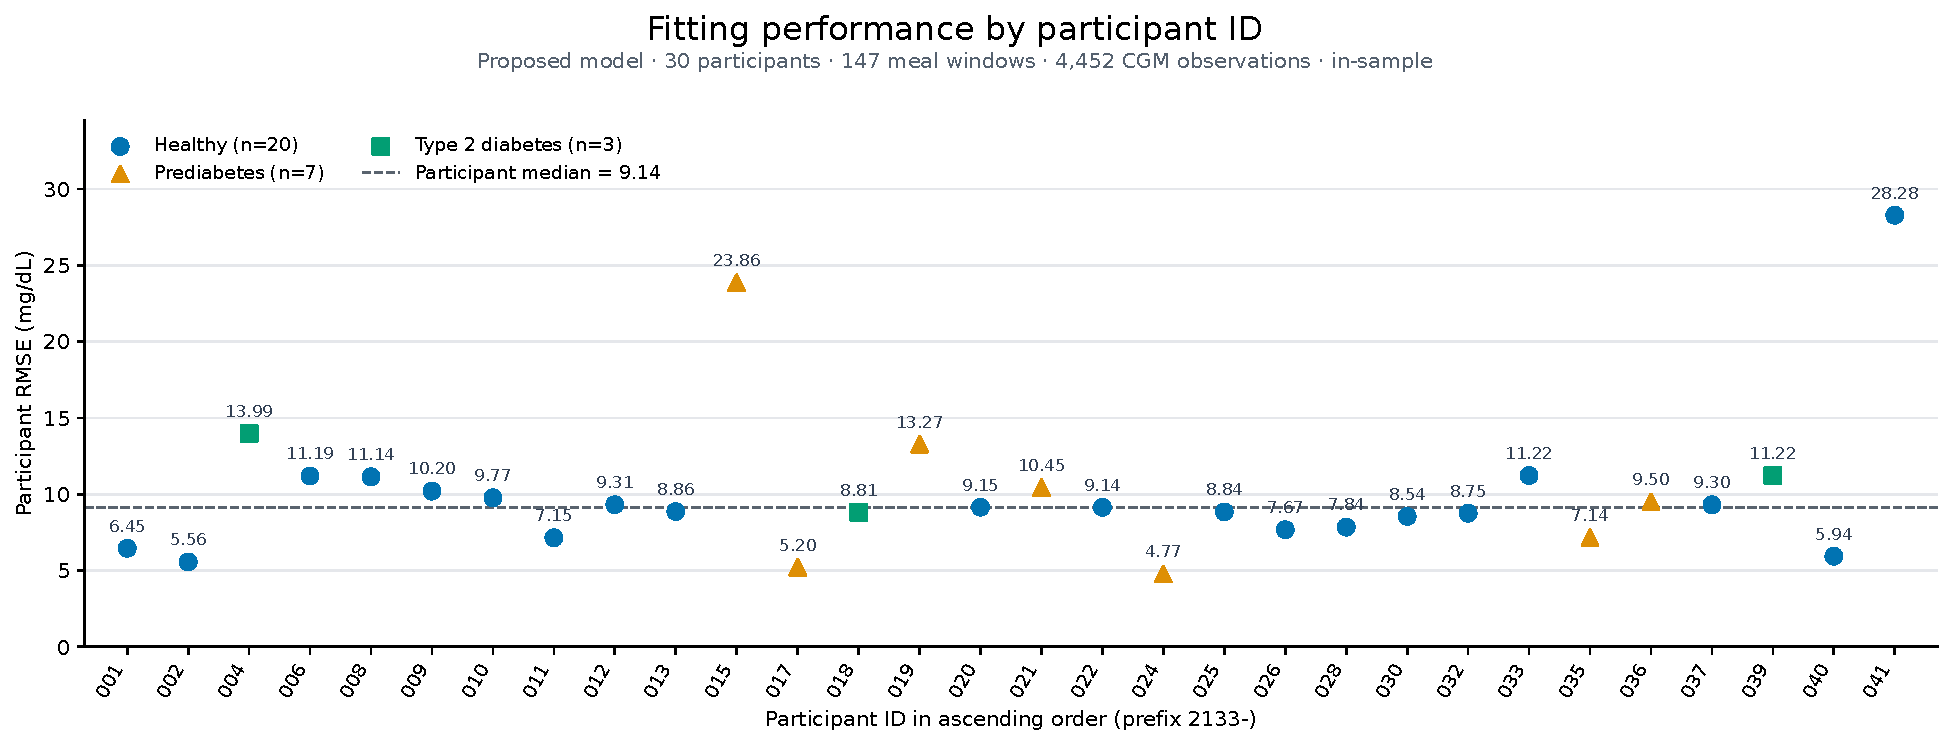
\includegraphics[width=\textwidth]{outputs/figures/figure_8_fit_by_id.pdf}
\caption{Participant-level fitting performance in ascending participant-ID order. All 30 fitted participants, 147 meal windows and 4,452 CGM observations are included. For each participant, RMSE is computed from all their fitted meal observations as $\sqrt{N_i^{-1}\sum_{e,t}(\widehat G_{iet}-G_{iet})^2}$, without observation weights. Points are colored and shaped by clinical status; numeric labels show RMSE in mg/dL. The dashed horizontal line is the median of participant RMSE values, not pooled RMSE. IDs are equally spaced in sorted order, with no implication of a continuous covariate. These are in-sample errors, including meal-time observations used for initialization; no participant is removed based on fitting quality.}
\label{fig:fit-by-id}
\end{figure*}

\begin{figure*}[t]
\centering
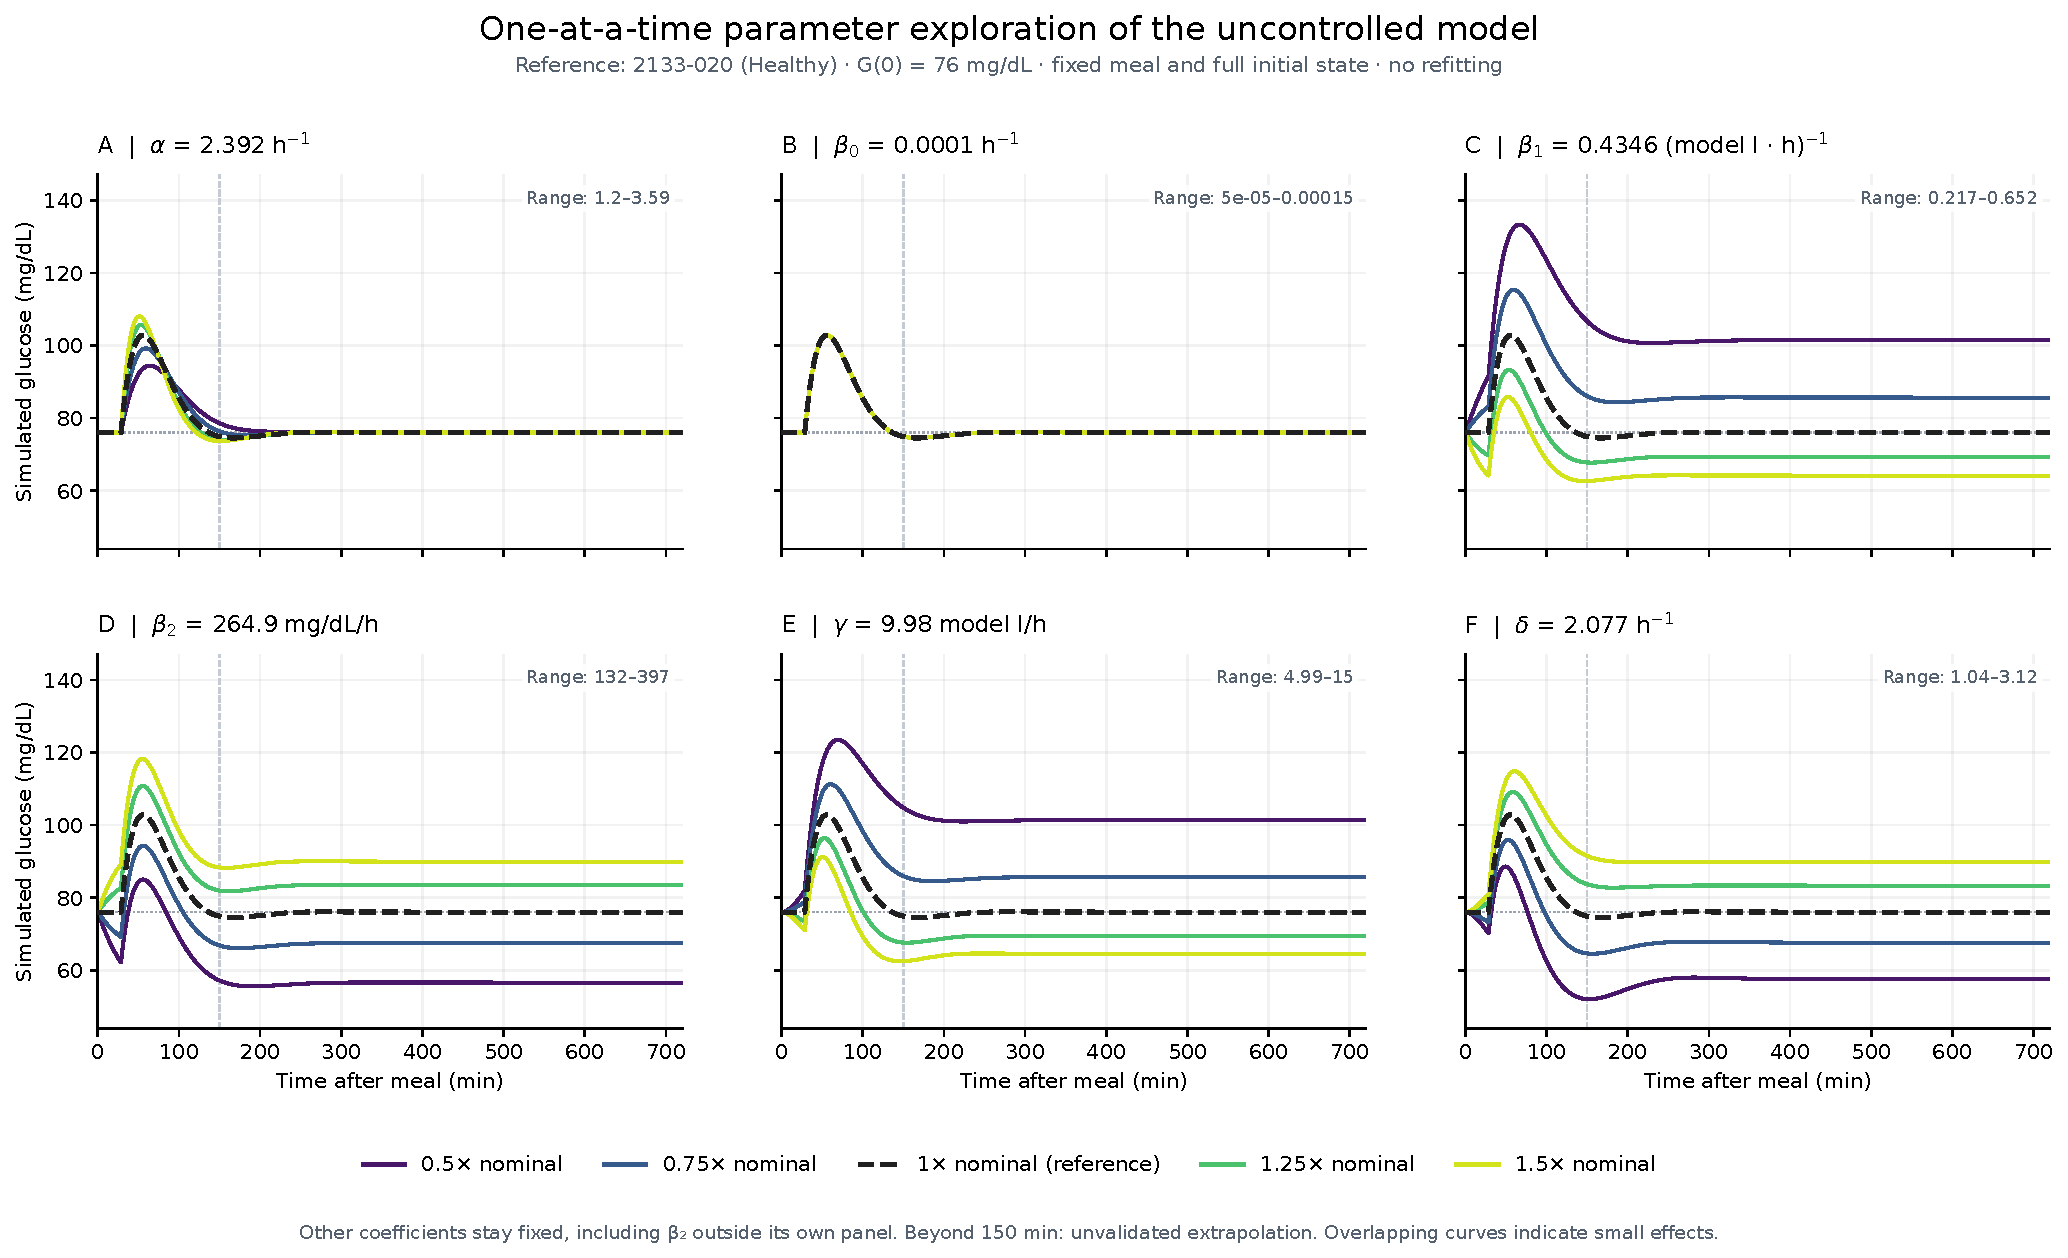
\includegraphics[width=\textwidth]{outputs/figures/figure_9_parameter_sweep.pdf}
\caption{One-at-a-time numerical exploration of the implemented uncontrolled model. The nominal coefficient vector is taken from fitted participant 2133-020 (Healthy); the reference-selection rule is recorded in the experiment metadata. Each coefficient is multiplied by 0.5, 0.75, 1, 1.25, 1.5, while all other coefficients remain fixed. The dashed black curve is the nominal response. The same initial digestive glucose, modeled glucose and quick-insulin state are used for every scenario; initial insulin is not re-equilibrated after perturbation. Nominal $\beta_2$ is derived from the fitted equilibrium constraint and then frozen, except in its own panel, where it is perturbed independently for this dynamical experiment only. Thus the experiment does not impose the fitting-stage equilibrium constraint on every perturbed coefficient vector. Horizontal dotted lines indicate nominal initial glucose; vertical dashed lines, when shown, mark the 150-minute endpoint of the fitting windows. Later behavior is unvalidated extrapolation. Multipliers are not clipped to optimization bounds; out-of-bound scenarios are flagged in the exported tables. The curves are not confidence bands, calibrated physiological interventions, or evidence of clinical efficacy.}
\label{fig:parameter-sweep}
\end{figure*}

\paragraph{Reproducible simulation settings.}
Nominal coefficients: $\alpha$=2.39194, $\beta_0$=0.000100049, $\beta_1$=0.434646, $\beta_2$=264.869, $\gamma$=9.98028, $\delta$=2.07744. Initial states are $D(0)=0$, $G(0)=76$ mg/dL and $I_q(0)=1.37533$ model units. Digestive-glucose amplitude is 59.8322, injected after an absorption delay of 28.5416 minutes; these are the reference participant's median fitted event amplitude and delay. The horizon is 12 hours, with nominal output spacing of 1 minute(s), plus the absorption instant and endpoint. Fixed constants are $K=120$ mg/dL and $I_b=1$ model units; external control is zero. Time in the equations is in hours; insulin is dimensionless and is not a clinical dose.

\paragraph{Scope of the dynamical analysis.}
The export includes the positive no-meal equilibrium and the eigenvalues of its exact three-state Jacobian for each coefficient vector. Negative real parts indicate local asymptotic stability of that equilibrium, while a complex pair allows damped oscillatory linearized modes. Neither a complex pair nor a finite simulated trajectory establishes a sustained oscillation, a limit cycle, or a global stability result. The analysis concerns one fitted reference scenario, not global parameter sensitivity or parameter identifiability.
